\section{SCD}
\thispagestyle{fancy}

Etter arbeidet med å få hovudblokkene på plass var det naturleg å sette seg ned å planlegge korleis vi ønska å knytte desse blokkene opp i mot anlegget. 
Vi valte da å starte med å lage eit System Control Diagram (SCD) over anlegget. 
Eit SCD er ein grafisk representasjon av anlegget, som visar komponentane i anlegget og deira funksjon, forbindelsar og struktur. 
IEC PAS 63131 standaren gir oss retningslinjene for utforming av diagrammet.


\begin{figure}[htbp]
    \centering
    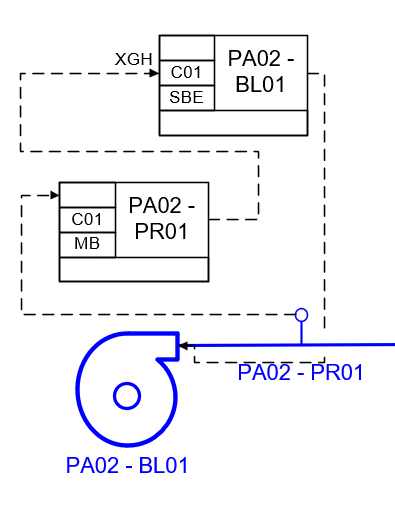
\includegraphics[width=0.35\textwidth]{Bilder/Visio_eksempel.png}
    \caption{Utsnitt frå SCD}\label{fig:SCD eksempel}    
\end{figure}


